%% LyX 2.1.1 created this file.  For more info, see http://www.lyx.org/.
%% Do not edit unless you really know what you are doing.
\documentclass[twocolumn,english,review, fleqn]{article}
\usepackage[OT1]{fontenc}
\usepackage[latin9]{inputenc}
\usepackage{geometry}
\geometry{verbose,tmargin=1in,bmargin=1in,lmargin=1in,rmargin=1in}
\usepackage{textcomp}
\usepackage{amsmath}
\usepackage{graphicx}
\usepackage{esint}
\usepackage[numbers]{natbib}

\makeatletter

%%%%%%%%%%%%%%%%%%%%%%%%%%%%%% LyX specific LaTeX commands.
%% Because html converters don't know tabularnewline
\providecommand{\tabularnewline}{\\}

\makeatother

\usepackage{babel}
\begin{document}

\title{Modeling Injected Interstitial Effects on Void Swelling in Self-Ion
Irradiation Experiments}


\author{M. P. Short%
\thanks{Dept. of Nuclear Science and Engineering, Massachusetts Institute
of Technology%
}%
\thanks{Corresponding Author: Tel: +1-617-347-7763, Email: hereiam@mit.edu%
}, D. R. Gaston%
\thanks{Idaho National Laboratory%
}, M. Jin%
\thanks{Dept. of Nuclear Science and Engineering, Massachusetts Institute
of Technology%
}, L. Shao%
\thanks{Dept. of Nuclear Engineering, Texas A\&M University%
}, F. A. Garner%
\thanks{Radiation Effects Consulting, LLC%
}}
\maketitle
\begin{abstract}
Heavy ion irradiations at high dose rates are often used to simulate
slow and expensive neutron irradiation experiments. However, many
differences in the resultant modes of damage arise due to unique aspects
of heavy ion irradiation. One such difference was recently shown in
pure iron to manifest itself as a double peak in void swelling, with
both peaks located away from the region of peak displacement damage
(DPA). In other cases involving a variety of ferritic alloys there
is often only a single peak in swelling vs. depth that is located
very near the ion-incident surface. We show that these behaviors arise
due to a combination of two separate effects: 1) suppression of void
swelling due to injected interstitials, and 2) preferential sinking
of interstitials to the ion-incident surface, which are very sensitive
to the irradiation temperature and atomic displacement rate. Care
should therefore be used in collection and interpreting of data from
the depth range outside the Bragg peak of ion irradiation experiments,
as it is shown to be more complex than previously envisioned.
\end{abstract}

\section{Introduction and Background}

Charged particle irradiation is frequently used to simulate the effect
of neutron irradiation on microstructural evolution of reactor structural
alloys, but is generally conducted at much higher displacement rates
in order to compress the time required to reach very high DPA levels
needed to observe phenomena such as neutron-induced void swelling
and embrittlement \citep{Was2007}. When optimized to maximize simulation
of void swelling, there is not a one-to-one correspondence between
microstructures observed under neutron and ion irradiation.

The primary reasons for this lack of correspondence are various consequences
of the increased DPA rate, very short ranges of the bombarding ion,
consequences of strong gradients in DPA rate along the ion range and
local defect imbalances arising from the bombarding ion \citep{Was2007,Garner1976,Garner1976a,Garner1976b,Packan1978,Lee1979,Garner1983,Bullen1984,Badger1985,Shao2014,Sindelar1985}.
Additionally, there are second-order effects such as ion-induced sputtering
\citep{Was2007,Johnston1973} and swelling-induced compressive states
in the thin irradiated film that produce a one-dimensional (not three-dimensional
as in the neutron irradiation case) flow of material toward the ion-incident
surface \citep{Garner1976c,Wolfer1979}. All of these processes can
be described as ``neutron-atypical'' effects.

Swelling of both neutron and ion irradiated metals has often been
shown to exhibit an incubation period before the onset of steady-state
swelling. This incubation period is strongly dependent on DPA rate
even in the absence of microchemical evolution \citep{Was2007,Garner1976a,Garner2012,Garner2010}.

In many alloys the onset of swelling requires that a microchemical
evolution involving segregation and precipitation first occur, but
the rate constants involved in the point defect and precipitation
sequences are usually rather different, producing different incubation
behavior at different DPA rates. The very short ion ranges not only
allow a strong influence of the specimen surface on defect loss and
dislocation loss that are atypical of neutron irradiation, but strong
gradients in DPA rate along the ion range provide an internal rate
effect on defect production \citep{Garner1976b}, and also provide
a driving force for elemental segregation along the ion path \citep{Pechenkin2013},
thereby influencing the microchemical evolution that often precedes
the onset of swelling.

Defect imbalances arising during ion irradiation arise from forward
scattering involved with ion-atom collisions and the spatial distribution
of injected ions, the latter having a very strong effect on swelling
that is designated as the injected interstitial effect \citep{Lee1979,Garner1983,Bullen1984,Badger1985,Shao2014,Sindelar1985}.
Garner et al. review the result of experiments conducted on pure iron
and various ferritic-martensitic alloys showing that the net effect
of the various neutron-atypical aspects is to produce a depth dependence
of void swelling that often bears no resemblance to the depth distribution
of the atomic displacement rate \citep{Garner2015}. Under some irradiation
conditions swelling only occurs near the specimen surface, and under
other conditions the swelling vs. depth is more complex, sometimes
producing two peaks, neither corresponding to the position of maximum
displacement rate \citep{Shao2014}.

Additionally, ion beams are often rastered to provide more spatially-uniform
damage fields while introducing non-uniform temporal distributions
compared to neutron irradiation. This latter effect is one of the
more important neutron-atypical processes that strongly affect swelling.
Since rastering and injected interstitials are both suppressive and
synergistic, especially on void nucleation, their interaction must
be recognized and factored into data analysis. Two recent papers demonstrate
the strong influence of rastering to suppress void swelling \citep{Gigax2015,Getto2015}.

If we could ignore all of these atypical influences and examine an
alloy that swells easily without much of an incubation period, one
might assume that the swelling vs. depth profile should mirror the
dose rate vs. depth profile, but this would be an incorrect assumption.
In general, alloys of even simple composition such as solute-free
Fe-Cr-Ni ternaries have been observed to exhibit a large range of
swelling vs. depth profiles, frequently with no resemblance to the
DPA vs. depth profile \citep{Sindelar1985,Johnston1976}.

In order to minimize these influences, the ion irradiation community
has learned to conduct irradiations on simple and complex alloys by
not rastering the beam and by choosing a narrow volume-slice at an
examination depth that minimizes the effects not only of the ion-incident
surface but especially the surprisingly strong injected interstitial
effect \citep{Garner1983,Shao2014}. However, the fullest utilization
of the ion irradiation technique would require an understanding of
the evolution of swelling vs. depth over the entire ion range, allowing
extraction of data over a much larger portion of the ion range. With
so many neutron-atypical processes operating simultaneously during
ion irradiation, a full understanding requires that a ``peel the
onion'' approach be used, starting with the simplest metals and alloys,
moving to more complex alloys, isolating and studying each neutron-atypical
process at each level of compositional and microstructural complexity.

Our approach to date has been to examine these neutron-atypical effects
first in annealed pure iron and cold-worked pure iron, focusing initially
on the rastering effect and the defect imbalance issues without the
added complexity arising from microchemical evolution, and then focusing
later on the same processes occurring in Fe-Cr binary alloys and then
solute-bearing Fe-Cr alloys.

In the first of these studies we focused on void swelling of annealed
pure iron in a beam-rastered irradiation, showing that the injected
interstitial effect indeed suppresses swelling \citep{Shao2014}.
In the second of these studies it was shown that rastering suppresses
swelling compared to non-rastered fixed beams \citep{Gigax2015}.
Figure 1 of Gigax's study (here reproduced in Figure \ref{fig:VoidNuc-Plots}c)
shows the two most salient features are the very strong impact of
the injected interstitial effect to suppress, to very high doses,
the void swelling throughout the injected ion range, and the appearance
of a double-peak swelling distribution in the region in front of injected
ion range. A similar observation was made in self-ion irradiations
on pure nickel many years earlier \citep{Bullen1984,Badger1985}.
Occasionally, double peaks are observed in other alloys, but the possibility
cannot be discounted that compositional segregation along the range
might be contributing to this observation. 

While the injected interstitial effect was not unexpected, the appearance
of a double peak in the fore-range of iron and nickel was rather surprising,
with the question entertained whether it might be an experimental
artifact or a real characteristic of ion irradiation. In this paper
we model the time-dependent development of depth-dependent void swelling
in annealed pure iron as a function of irradiation temperature and
accumulated dose produced during non-rastered irradiation with 3.5
MeV Fe ions. It is found that both the double peak and the injected
interstitial suppression effects are consequences of the defect imbalance
effect, reproducing the observed behavior. This model can then be
used to forecast swelling behavior in pure iron and possibly more
complex iron-base alloys for other temperatures, DPA rates, ion energies,
rastering frequencies, etc. In particular, the double-peak is predicted
to only manifest itself within a narrow window ({\raise.17ex\hbox{$\scriptstyle\sim$}}30K)
of temperature, which may explain some of its previous elusiveness.


\section{Methodology}

A fully coupled implementation of the point defect kinetics equations
in the form of Equations 10 and 11 in \citep{Golubov2012} was implemented
in MOOSE \citep{Gaston2009}, the Multiphysics Object Oriented Simulation
Environment, a finite element method framework. By fully coupled,
we refer to the definition of all equations and material properties
as functions of all possible independent variables (defect concentrations,
temperature, ion beam current) rather than using any numerically convenient
assumptions of constant or simplified material properties. Only the
initial stages of point defect creation and subsequent void nucleation
rates at zero time were studied, further stabilization and growth
of voids typical of cluster dynamics simulations was not considered
in this study.

The reader should therefore note what this study is and what it is
not. It is a simple demonstration that accounting for a tiny fraction
of injected interstitials greatly changes the qualitative form of
the void swelling distribution. This study is not meant to be quantitative
in any way, nor does it predict true, time-dependent microstructure
evolution. Other recent studies using normal rate theory (NRT) and
the production bias model (PBM) \citep{Golubov2012}, which accounts
for the creation and evolution of self-interstitial atom (SIA) clusters,
treat radiation-induced microstructural evolution in a more quantitative
manner.


\subsection{Equational Framework}

The point defect kinetics equations were implemented as follows:

\noindent \begin{flushleft}
\[
\mathit{\frac{\partial C_{v}}{\partial t}}=\mathit{f_{survive}K_{0}}
\]
\begin{equation}
\mathit{-K_{\bot,v}\rho_{\bot}C_{v}-K_{iv}C_{v}C_{i}+D_{v}\nabla^{2}C_{v}}\label{eq:Point-Defects-Vacancies}
\end{equation}

\par\end{flushleft}

\noindent \begin{flushleft}
\[
\mathit{\frac{\partial C_{i}}{\partial t}}=\mathit{\left[f_{survive}\left(1-f_{i-cluster}\right)K_{0}+K_{II}\right]}
\]
\begin{equation}
\mathit{-K_{\bot,i}\rho_{\bot}C_{i}-K_{iv}C_{i}C_{v}+D_{i}\nabla^{2}C_{i}}\label{eq:Point-Defects-Interstitials}
\end{equation}

\par\end{flushleft}

\noindent where $\mathit{C_{v}}$ and $\mathit{C_{i}}$ are the spatially-dependent
concentrations of vacancies and interstitials in $\mathrm{\left[\frac{\#}{nm^{3}}\right]}$,
$\mathit{f_{survive}}$ is the intracascade point defect survival
fraction (the true fraction of remaining point defects after the damage
cascade quenches \& anneals), $\mathit{K_{0}}$ is the point defect
source term from binary collisions in $\mathrm{\left[\frac{\#}{nm^{3}-s}\right]}$,
$\mathit{K_{II}}$ is the injected interstitial source term in $\mathrm{\left[\frac{\#}{nm^{3}-s}\right]}$,
$\mathit{K_{\bot}}$ is the dislocation sink rate constant in $\left[\frac{1}{s}\right]$,
$\mathit{K_{iv}}$ is the vacancy/interstitial recombination rate
constant in $\left[\frac{nm^{3}}{\#-s}\right]$, and $\mathit{D_{v}}$
\& $\mathit{D_{i}}$ are the diffusivities of vacancies and interstitials
in $\mathrm{\left[\frac{nm^{2}}{s}\right]}$. All rate constants,
diffusivities, and point defect concentrations are spatially dependent
in one dimension on local state variables and defect concentrations.
Here, an aspect of the PBM was used to assume that a fraction of interstitials
immediately form highly mobile SIA clusters within each damage cascade
\citep{Golubov2012}, which diffuse so quickly in one dimension that
they are eliminated from localized recombination and sinking. The
SIA cluster concentration is therefore not tracked in this model.

The term $\mathrm{K_{0}}$ was calculated using the SRIM-2010 code
\citep{Ziegler2010}, with simulation parameters as shown in Table
\ref{tab:SRIM-simulation-parameters}.
\begin{table}
\noindent \begin{centering}
\begin{tabular}{|c|c|c|}
\hline 
\textbf{SRIM Parameter} & \textbf{Value} & \textbf{Unit}\tabularnewline
\hline 
\hline 
Ion Type & $\mathrm{Fe^{++}}$ & ---\tabularnewline
\hline 
Target & Pure Fe & ---\tabularnewline
\hline 
Ion Energy & 3.5 & MeV\tabularnewline
\hline 
Number of Ions & 500,000 & \#\tabularnewline
\hline 
Target Density & 7.85 & $\mathrm{\frac{g}{cm^{3}}}$\tabularnewline
\hline 
Target Thickness & 3 & $\mathrm{\mu m}$\tabularnewline
\hline 
\end{tabular}
\par\end{centering}

\protect\caption{\label{tab:SRIM-simulation-parameters}SRIM simulation parameters
used to generate the point defect source term in this study}


\end{table}
 These parameters were chosen to match those used in the experiments
of Shao et al. \citep{Shao2014}. SRIM was run in ``quick calculation''
mode using the Kinchin-Pease model, to avoid recently discovered anomalies
in its full-cascade model \citep{Stoller2013}. Also, because the
random number seed in SRIM does not change automatically, 50 separate
simulations each containing 10,000 flown ions were averaged using
a script%
\footnote{All scripts, input files, and output files used in this study are
permanently posted on our Github repository: \citep{GitHub2015}%
} to obtain smooth profiles of both the DPA rate and the injected interstitial
rate as a function of distance from the free surface.

\begin{figure}
\noindent \begin{centering}
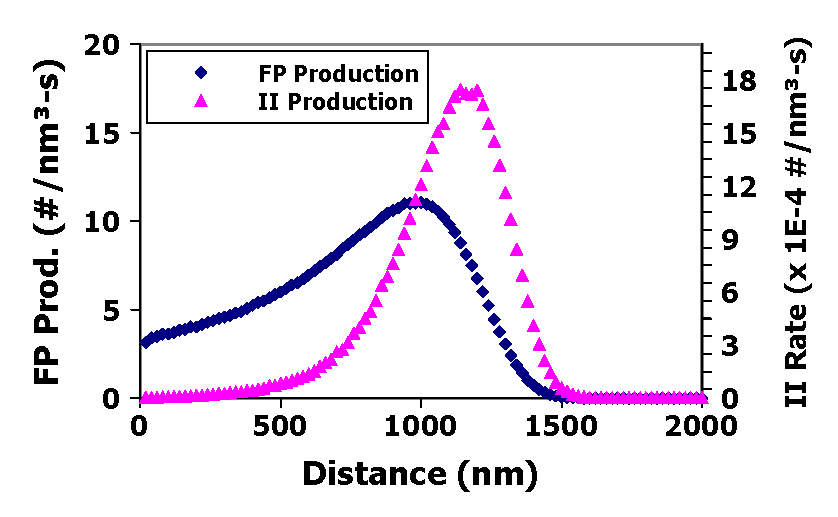
\includegraphics[width=0.9\columnwidth]{Figures/Defect-Production}\protect\caption{\label{fig:SRIM-Rates}Frenkel pair (FP) and injected interstitial
(II) production rates, as calculated by SRIM. Note the peak ballistic
damage rate at 1000\,nm.}

\par\end{centering}

\end{figure}
The VACANCY.TXT and RANGE.TXT files from SRIM (shown in Figure \ref{fig:SRIM-Rates}),
which give $\frac{Vacancies}{\textrm{\AA-ion}}$ and $\frac{injected\thinspace ions}{cm}$,
respectively, were converted to data files giving defect production
and interstitial injection rates. The ballistic Frenkel pair (FP)
production rate was multiplied by the experimentally measured beam
current (200nA) and dividing by the beam area (1mm in diameter) in
terms of the ionic flux:

\[
K_{0_{FPs}}\left(x\right)\left[\frac{Vac.}{nm^{3}-sec}\right]
\]


\[
=\left(K_{PKAs}+K_{Recoils}\right)_{SRIM}\left[\frac{Vac.}{\textrm{\AA}-ion}\right]
\]
\[
*\frac{10\thinspace\textrm{\AA}}{1\thinspace nm}*\frac{1\thinspace Fe^{+2}\thinspace ion}{2\thinspace e^{-}}*200nA*\frac{1\thinspace\frac{e^{-}}{sec}}{1.6\cdot10^{-10}\thinspace nA}
\]
\begin{equation}
*\frac{1}{\pi\left(5\cdot10^{5}nm\right)^{2}}=7.96\left(K_{PKAs}+K_{Recoils}\right)_{SRIM}\label{eq:Ion-Flux}
\end{equation}
Simultaneously, the spatially dependent ion range distribution from
SRIM was converted to total injected interstitials (II) per nm, by
also multiplying by the beam current density:{\small{}
\[
K_{0_{II}}\left(x\right)\left[\frac{II}{nm^{3}-sec}\right]=RANGE_{SRIM}\left[\frac{\frac{ions}{cm^{3}}}{\frac{ions}{cm^{2}}}\right]*\frac{1\thinspace cm}{10^{7}\thinspace nm}
\]
\[
*\frac{1\thinspace Fe^{+2}\thinspace ion}{2\thinspace e^{-}}*200nA*\frac{1\thinspace\frac{e^{-}}{sec}}{1.6\cdot10^{-10}\thinspace nA}
\]
\begin{equation}
*\frac{1}{\pi\left(5\cdot10^{5}nm\right)^{2}}=RANGE_{SRIM}\left(x\right)*\left(7.96\cdot10^{-8}\right)\label{eq:Ion-Ranges}
\end{equation}
}{\small \par}

Next, the dislocation sink rate constant was calculated by first finding
half the average distance between dislocations $\left(\frac{1}{2}d_{\bot}\right)$
based on the dislocation density $\left(\rho_{\bot}\right)$:
\begin{equation}
\frac{1}{2}d_{\bot}=\frac{1}{\sqrt{\pi\rho_{\bot}}}\label{eq:Dislocation-Half-Distance}
\end{equation}
and then using it to calculate the dislocation sink rate constant:
\begin{equation}
K_{\bot,\left(v,i\right)}=\frac{2\pi D_{\left(v,i\right)}}{ln\left(\frac{\frac{1}{2}d_{\bot}}{r_{\bot\left(v,i\right)}}\right)}\label{eq:Dislocation-Sink-Rate}
\end{equation}
where $\mathit{r_{\bot}}$ is the \emph{core size} of the dislocation
for each type of defect, or the approximate radius of capture should
a particular defect stray within this radius. The recombination rate
constant was calculated as follows:
\begin{equation}
K_{iv}=\frac{z_{iv}V_{Fe}\left(D_{v}+D_{i}\right)}{a_{Fe}^{2}}\label{eq:Recombination-Rate-Constant}
\end{equation}
where $\mathit{a_{Fe}}$ is the temperature-dependent lattice parameter
of iron, $\mathit{V_{Fe}}$ is the temperature-dependent atomic volume
of iron, and $\mathit{z_{iv}\sim500}$ \citep{Was2007}. Temperature-dependent
diffusivities were calculated using an Arrhenius relation:
\begin{equation}
D_{\left(v,i\right)}=D_{0}e^{\left(\frac{-E_{A_{\left(v,i\right)}}}{k_{B}T}\right)}\label{eq:Diffusivity-Equation}
\end{equation}
where $\mathit{D_{0}}$ is a diffusivity prefactor, $\mathrm{E_{A_{\left(v,i\right)}}}$are
the activation energies for point defect migration in eV, \emph{$\mathit{k_{B}}$}
is the Boltzmann constant $\mathrm{\left(8.62\cdot10^{-5}\,\frac{eV}{K}\right)}$,
and \emph{T} is the temperature in Kelvin. The atomic volume of iron
$\left(V_{Fe}\right)$ was found from molecular dynamics simulations
from \citep{Mendelev2009}:{\small{}
\begin{equation}
V_{Fe}\left[nm^{3}\right]=1.93559\cdot10^{-10}T^{2}+2.68634\cdot10^{-7}T+0.0116954\label{eq:Atomic-Volume}
\end{equation}
}The thermal vacancy concentration $\mathit{C_{v}^{*}}$ as a function
of temperature was found using molecular dynamics simulations from
\citep{Mendelev2009}:
\begin{equation}
C_{V}^{*}\,\left[\frac{\#}{nm^{3}}\right]=N_{Fe}\cdot10^{\left[-44.5997+5.73698\cdot ln\left(T-376.952\right)\right]}\label{eq:Thermal-Vacancies}
\end{equation}
where $\mathit{N_{Fe}}$ is the atomic number density of iron, given
by the following formula:
\begin{equation}
N_{Fe}\,\left[\frac{\#}{nm^{3}}\right]=\frac{\rho_{Fe}\cdot N_{A}}{\left(\frac{10^{21}\, nm^{3}}{1\, cm^{3}}\right)\cdot MM_{Fe}}\label{eq:Number-Density}
\end{equation}
where $\rho_{Fe}$ is the density of pure iron $\left(7.85\,\frac{g}{cm^{3}}\right)$,
$\mathit{N_{A}}$ is Avogadro's number $\left(6.02\cdot10^{23}\right)$,
and $\mathit{MM_{Fe}}$ is the molar mass of natural iron $\left(55.865\,\frac{g}{mol}\right)$.
Table \ref{tab:Material-property-parameters} summarizes material
property constants and parameters assumed in this study.
\begin{table}
\noindent \begin{centering}
\begin{tabular}{|c|c|c|c|}
\hline 
Property & Value & Unit & Source\tabularnewline
\hline 
\hline 
T & 450 & \textdegree C & Expt.\tabularnewline
\hline 
Beam Current & 200 & nA & Expt.\tabularnewline
\hline 
Beam Area & 1 & $\mathrm{mm^{2}}$ & Expt.\tabularnewline
\hline 
Peak DPA Rate & $\mathrm{4.6\cdot10^{-3}}$ & $\frac{DPA}{sec}$ & Expt.\tabularnewline
\hline 
$\mathrm{D_{0_{v}}}$ & 8.016$\cdot10^{11}$ & $\frac{nm^{2}}{s}$ & \citep{Borodin2007}\tabularnewline
\hline 
$\mathrm{D_{0_{i}}}$ & 2.09$\cdot10^{11}$ & $\frac{nm^{2}}{s}$ & \citep{Soneda2001}\tabularnewline
\hline 
$\mathrm{E_{m_{v}}}$ & 0.86 & eV & See Text\tabularnewline
\hline 
$\mathrm{E_{m_{i}}}$ & 0.17 & eV & \citep{Soneda2001}\tabularnewline
\hline 
$\mathit{r_{\bot_{v}}}$ & 1.2 & nm & \citep{Shastry1999}\tabularnewline
\hline 
$\mathit{r_{\bot_{i}}}$ & 3.6 & nm & \citep{Shastry1999}\tabularnewline
\hline 
$\rho_{\bot}$ & $\mathrm{10^{-5}}$ & $\frac{\#}{nm^{2}}$ & \citep{Bhadeshia2011}\tabularnewline
\hline 
$\mathrm{a_{Fe}}$ & 0.286 & nm & at 450\textdegree C\tabularnewline
\hline 
$\mathit{f_{survive}}$ & 25 & \% & \citep{Malerb2006}\tabularnewline
\hline 
$\mathit{f_{i-cluster}}$ & 30 & \% & \citep{Golubov2012}\tabularnewline
\hline 
\end{tabular}
\par\end{centering}

\protect\caption{\label{tab:Material-property-parameters}Material property parameters
used in this study}


\end{table}
 The migration energy of vacancies in 99.999\% iron was chosen to
be higher than the 0.66\,eV value for atomically pure iron \citep{Soneda2001}
found by molecular dynamics or 0.55\,eV found experimentally \citep{Wollenberger1996},
to account for realistic impurities and defect-solute binding. It
was also chosen to be lower than vacancy migration energies for other
BCC steels, such as the Russian alloys ChS-68 (1.08\,eV) or EK-164
(0.98\,eV) \citep{Kozlov2014}. The actual value is known to vary
between 0.75-1.4\,eV for carbon-doped $\alpha$-Fe \citep{Takaki1983},
as the binding energy of vacancy-carbon complexes at Stage III temperatures
has been measured at 1.1\,eV. This was the only fitting parameter
in this study, and was tuned to 0.86\,eV to induce double peak formation.
The sensitivity of the results to this parameter are discussed in
later sections of this manuscript.

To obtain the zero-time void nucleation rate behavior, the vacancy
supersaturation is first calculated as follows:
\begin{equation}
S_{v}=\frac{D_{v}C_{v}-D_{i}C_{i}}{D_{v}C_{v}^{*}}\label{eq:Supersaturation}
\end{equation}
This study is not a quantification of the true void nucleation rate,
but rather an estimation of relative effects. Therefore the general
\emph{shape} of a post-processed supersaturation vs. void nucleation
rate curve derived from \citep{Katz1971}, which is fully summarized
in \citep{Wiedersich1972}. It is worth noting here that while the
void nucleation rate at very low dose and the void swelling rates
are not directly comparable, their qualitative shapes are expected
to be similar. It is well known that voids and void nuclei constitute
additional point defect sinks with their own biases, more appropriately
treated using Master equation \citep{Golubov2012} or cluster dynamics
\citep{Jourdan2014} approaches.

This underscores the point that the quantity of interest in this study
is the \emph{spatially dependent vacancy supersaturation}, of which
the zero-time void nucleation rate is a very sensitive function. This
function does not vary considerably in shape over a very wide temperature
range of 200K \citep{Katz1971,Wiedersich1972}. Therefore, the same
void nucleation rate curve shape is used for different conditions
and materials to illustrate the strong effect of the more subtle variations
in vacancy supersaturation. The curve used was for the case of Ni
at 427\textdegree C, with an interstitial/vacancy arrival ratio of
$\frac{\beta_{i}}{\beta_{v}}=0.9$. The equation is as follows:
\begin{equation}
log\left(J_{V}\right)=5.41547\thinspace log\left(S_{v}\right)-14.6586\label{eq:Void-Nucleation-Rate}
\end{equation}
where \emph{$\mathit{J_{V}}$} is the void nucleation rate in $\mathrm{\left[\frac{\#}{nm^{3}-s}\right]}$.


\subsection{Finite Element Formulation}

A one-dimensional, time-dependent finite element simulation tool,
centered around Equations \ref{eq:Point-Defects-Vacancies}-\ref{eq:Number-Density},
was developed using MOOSE \citep{Gaston2009}. An initial mesh size
of 2\,$\mu m$ consisting of 200 elements was chosen, as the ultimate
range of 3.5\,MeV iron ions in iron was found to be 1.5\,$\mu m$,
and the SRIM data for damage production and ion range were binned
into 100 spatial nodes. Zero concentration Dirichlet boundary conditions
were assumed at the ends of the mesh for simplicity, and because a
free surface acts as a very strong sink for defects. The SolutionDT
adaptive time stepping algorithm was used to accelerate simulations
when appropriate. SolutionDT works by increasing the time step by
a factor of 1.5 if the current time step's solution was found to deviate
very little from the previous time step.

The single matrix preconditioner (SMP) was employed to assure computational
efficiency, allowing` one to only specify certain off-diagonal Jacobian
terms of the discretized partial differential equations (PDEs) in
the problem. This preconditioner was chosen to strike a compromise
between solving a Jacobian-free problem, which utilizes little computational
overhead before each solve but requires more iterations to converge,
and fully inverting the solution matrix, which yields an exact solution
after prohibitively long times. The total residuals for each variable
$\mathit{C_{v}}$ and $\mathit{C_{i}}$ are derived from the weak
forms of Equations \ref{eq:Point-Defects-Vacancies}-\ref{eq:Point-Defects-Interstitials},
which were implemented as follows:
\[
\left|r^{2}\right|_{C_{v}}=0=\underset{\Omega}{\int}\left[\psi_{I}\frac{\partial C_{v}}{\partial t}-\psi_{I}\left(f_{s}K_{0}\right)+\psi_{I}K_{\bot_{v}}C_{v}\right]
\]
\begin{equation}
+\underset{\Omega}{\int}\left[\psi_{I}K_{iv}C_{v}C_{i}+D_{v}\nabla\psi_{I}\nabla C_{v}\right]+\underset{\Gamma}{\int}\left[D_{v}\psi_{I}\nabla C_{v}\cdot\overrightarrow{n}\right]\label{eq:Weak-PDE-Vacancies}
\end{equation}
\[
\left|r^{2}\right|_{C_{i}}=0=\underset{\Omega}{\int}\left[\psi_{I}\frac{\partial C_{i}}{\partial t}-\psi_{I}\left(\left(f_{s}K_{0}\right)+K_{II}\right)\right]
\]
{\small{}
\begin{equation}
+\underset{\Omega}{\int}\left[\psi_{I}K_{iv}C_{i}C_{v}+\psi_{I}K_{\bot_{i}}C_{i}+D_{i}\nabla\psi_{I}\nabla C_{i}\right]+\underset{\Gamma}{\int}\left[D_{i}\psi_{I}\nabla C_{i}\cdot\overrightarrow{n}\right]\label{eq:Weak-PDE-Interstitials}
\end{equation}
}where $\psi_{I}$ is a particular test function, $\Omega$ is the
domain volume, $\Gamma$ represents the boundaries of the domain $\Omega$,
and $\overrightarrow{n}$ is the surface normal vector at each boundary
$\Gamma$. Reference \citep{Gaston2009} contains a more thorough
description of the weak form equation development in the MOOSE framework.
The on-diagonal and off-diagonal Jacobians for Equations \ref{eq:Weak-PDE-Vacancies}-\ref{eq:Weak-PDE-Interstitials}
were defined as follows:
\[
\frac{\partial C_{v}}{\partial C_{v}\left(I\right)}=-\psi_{I}\phi_{J}\frac{\partial\left[\frac{\partial C_{v}}{\partial t}\right]}{\partial C_{v}}
\]
\begin{equation}
+\psi_{I}K_{iv}C_{i}\phi_{J}+\psi_{I}K_{\bot_{v}}\phi_{J}+D_{v}\nabla\phi_{J}\nabla\psi_{I}\label{eq:Jacobian-Vacancies}
\end{equation}
\[
\frac{\partial C_{i}}{\partial C_{i}\left(I\right)}=-\psi_{I}\phi_{J}\frac{\partial\left[\frac{\partial C_{i}}{\partial t}\right]}{\partial C_{i}}
\]
\begin{equation}
+\psi_{I}K_{iv}C_{v}\phi_{J}+\psi_{I}K_{\bot_{i}}\phi_{J}+D_{i}\nabla\phi_{J}\nabla\psi_{I}\label{eq:Jacobian-Interstitials}
\end{equation}
\begin{equation}
\frac{\partial C_{v}}{\partial C_{v}\left(J\right)}=\psi_{I}K_{iv}\phi_{J}C_{v}\label{eq:OffDiag-Jacobian-Vacancies}
\end{equation}
\begin{equation}
\frac{\partial C_{i}}{\partial C_{i}\left(J\right)}=\psi_{I}K_{iv}\phi_{J}C_{i}\label{eq:OffDiag-Jacobian-Interstitials}
\end{equation}
where \emph{I} is the index (node value) for the shape function $\psi_{I}$
under consideration, \emph{J} is an index for a particular trial function
$\phi_{J}$ under consideration. An implicit Euler time step method
was used, resulting in $\mathrm{\frac{\partial\frac{\partial u}{\partial t}}{\partial u}=\frac{1}{\Delta t}}$,
where \emph{u }is the variable under consideration. Note that the
only terms that contain an off-diagonal Jacobian entry in the solution
matrix are coupled terms, where two or more variables in the constitutive
PDEs are found in the same term. The only terms containing a non-zero
off-diagonal Jacobian entry are the defect recombination terms, as
they explicitly contain both $C_{v}$ and $C_{i}$, which are the
variables used in the PDEs in this framework.


\section{Results}

First, the results of intermediate calculations are given, followed
by simulation results meant to match the experiments of Shao et al.
\citep{Shao2014}. Next follows predictions for varied experimental
conditions. Results are given for two cases: with and without injected
interstitials, the latter case removing the $\mathit{K_{II}}$ term
from Equations \ref{eq:Point-Defects-Interstitials} and \ref{eq:Weak-PDE-Interstitials}.


\subsection{Defect Concentrations}

\begin{figure}
\noindent \begin{centering}
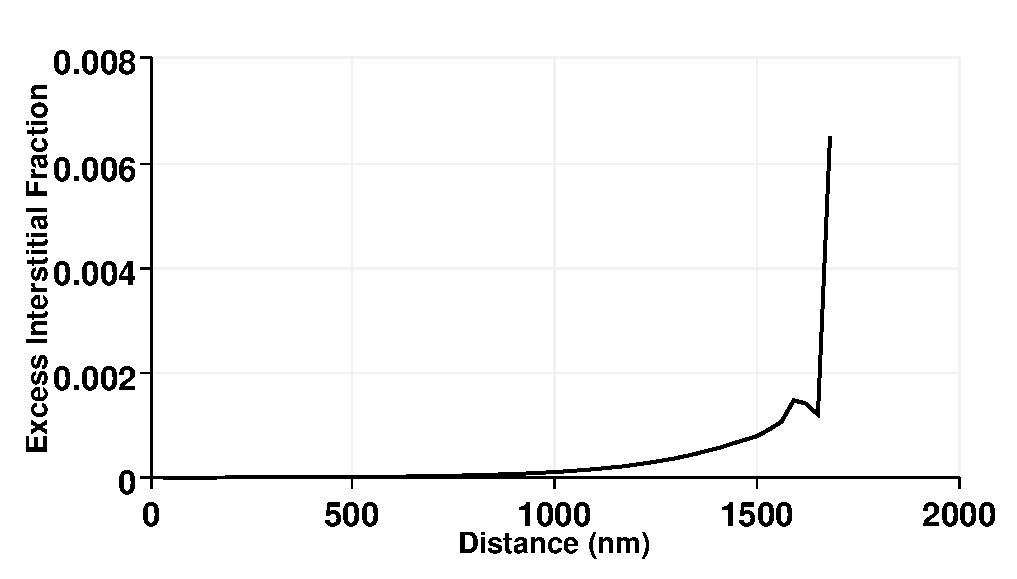
\includegraphics[width=0.9\columnwidth]{Figures/ExcessInt}\protect\caption{\label{fig:Excess-Interstitials}Spatially dependent excess interstitial
fraction with injected interstitials, peaking at a value of 0.7\%.
The bump in the curve at 1650~nm is an artifact of noise from the
SRIM simulation.}

\par\end{centering}

\end{figure}
Figure \ref{fig:Excess-Interstitials} shows a spatial plot of the
excess injected interstitial fraction, or the ratio of the total interstitial-to-vacancy
production rate minus one. The plot ends near the end of the FP production
region, as the excess injected interstitial fraction is invalid beyond
this region. 
\begin{figure}
\noindent \begin{centering}
\includegraphics[width=0.9\columnwidth]{Figures/Defect-Comparison}
\par\end{centering}

\noindent \centering{}\protect\caption{\label{fig:Defect-Plots}Spatially dependent defect concentrations,
without (dashed) and with (solid) injected interstitials}
\end{figure}
Figure \ref{fig:Defect-Plots} shows the quasi-steady state defect
concentrations for the cases with and without injected interstitials.
Even though the excess injected interstitial fraction shows a very
slight imbalance between defect production rates, in the hundreds
of ppm on average, the resulting steady-state defect concentrations
differ greatly. This imbalance, especially near the Bragg peak region
of the ions where SRIM calculates the most damage, causes a shift
in the damage peak towards the free surface. The effect of the free
surface itself, which is modeled as an undepletable sink with a zero
defect concentration, is also pronounced, preferentially removing
interstitials in the vicinity due to their higher mobility.


\subsection{Vacancy Supersaturation and Qualitative Void Nucleation Rate}

\begin{figure}
\noindent \begin{centering}
\includegraphics[width=0.9\columnwidth]{Figures/Supersat}
\par\end{centering}

\noindent \centering{}\protect\caption{\label{fig:SuperSat-Plots}Vacancy supersaturation, without (black
dashed) and with (solid red) injected interstitials}
\end{figure}
The resulting vacancy supersaturation curves for cases with and without
injected interstitials are shown in Figure \ref{fig:SuperSat-Plots}.
Two main features are of significant interest here. Firstly, the appearance
of a second peak in supersaturation, though small, is quite significant.
Secondly, the pull of the free surface, combined with a 55\% suppression
of vacancy supersaturation at the location of peak damage by injected
interstitials, ``exposes'' this second peak rather than inducing
it.

\begin{figure}
\noindent \begin{centering}
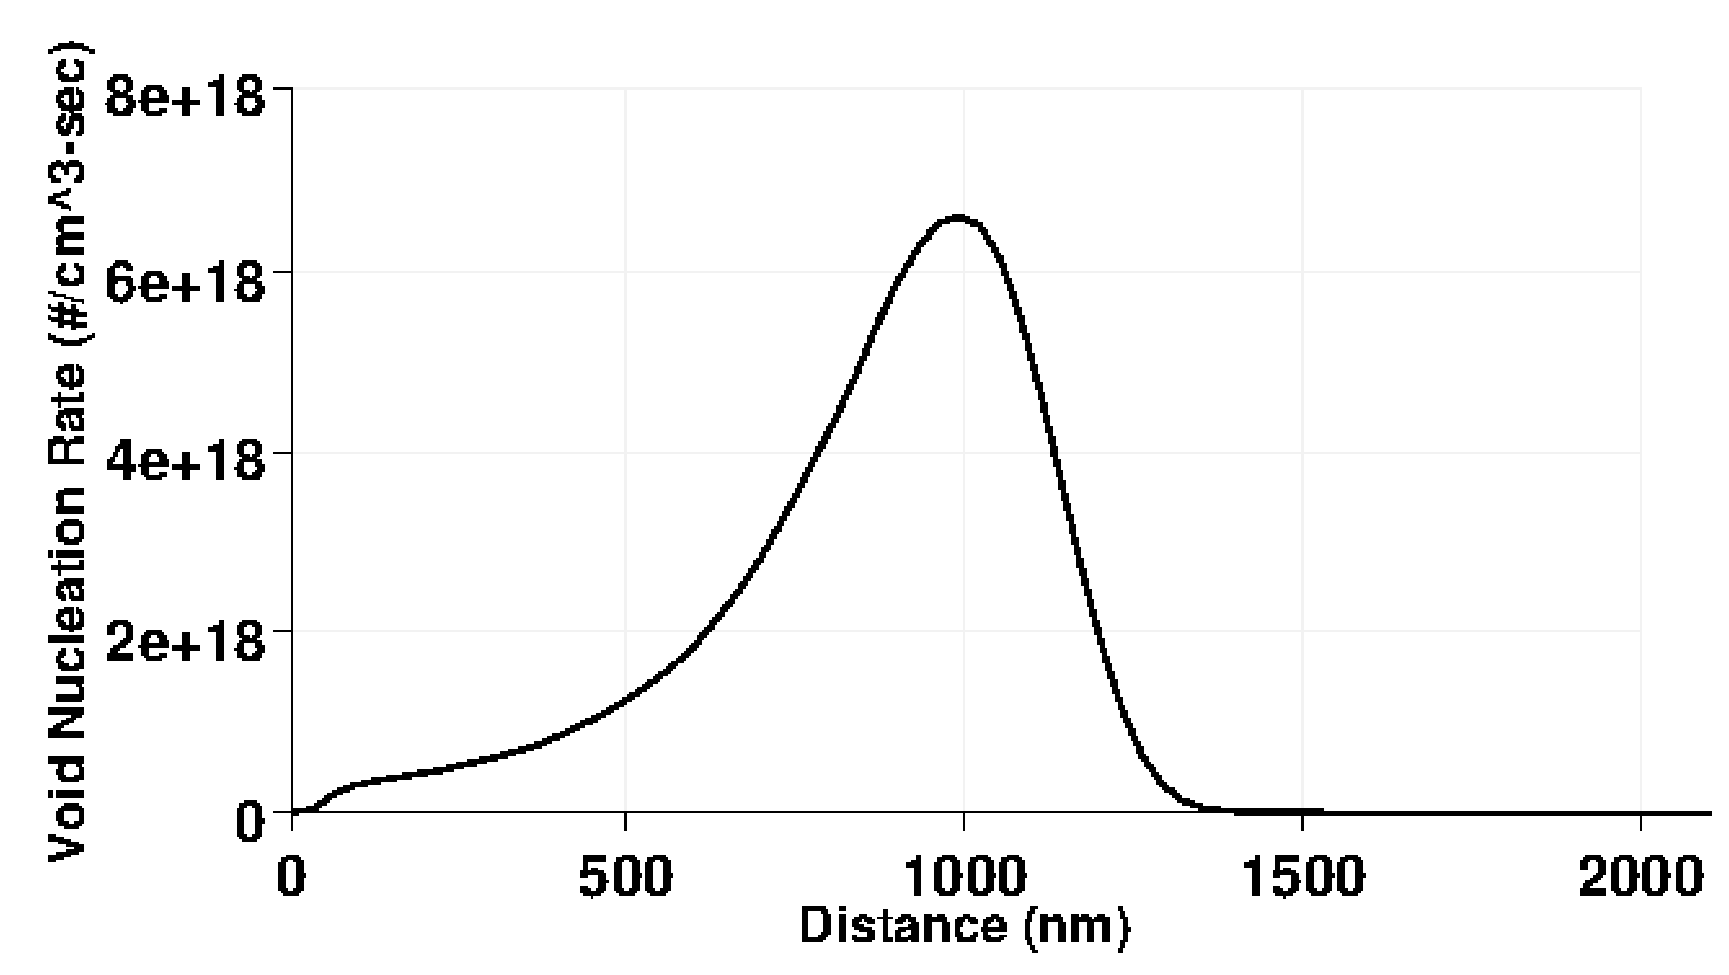
\includegraphics[width=0.9\columnwidth]{Figures/VoidNuc-NoII}
\par\end{centering}

\noindent \begin{centering}
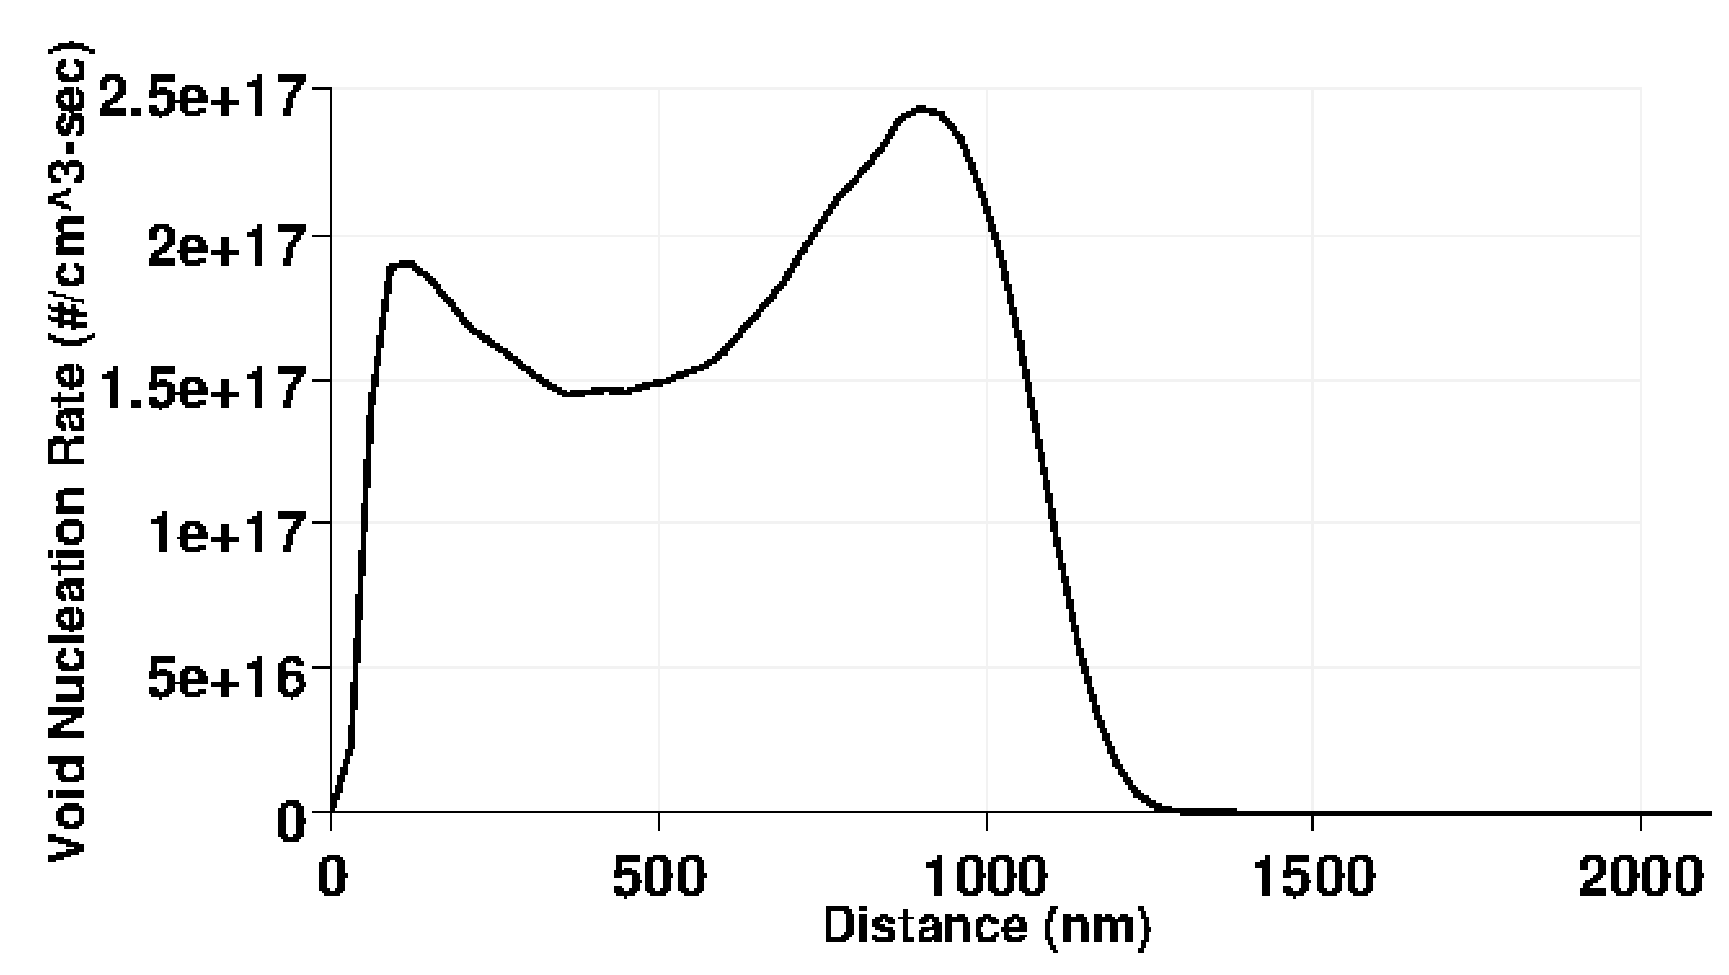
\includegraphics[width=0.9\columnwidth]{Figures/VoidNuc-II}
\par\end{centering}

\noindent \begin{centering}
\includegraphics[width=0.9\columnwidth]{Figures/Shao-Experiment}
\par\end{centering}

\noindent \centering{}\protect\caption{\label{fig:VoidNuc-Plots}Void nucleation rate curve shapes, without
(top) and with (middle) injected interstitials, compared to (bottom)
the experimental void swelling distribution observed in 3.5\,MeV
$\mathrm{Fe^{+2}}$ irradiation of pure iron \citep{Shao2014}}
\end{figure}
Void nucleation rates with and without injected interstitials are
shown in Figures \ref{fig:VoidNuc-Plots}a-b. The larger disparity
is due to the very high sensitivity of void nucleation rate to vacancy
supersaturation value, which can change by 10-15 orders of magnitude
for a 10x increase in vacancy supersaturation \citep{Katz1971}. The
case with injected interstitials is presented above matching experimental
data from \citep{Shao2014}, conducted under similar conditions as
those simulated in this study, showing better agreement compared to
the prediction without injected interstitials. However, the model
does not predict enough of a swelling peak shift towards the free
surface to match the experimental data. Also note how the presence
of injected interstitials shifts the peak supersaturation level and
void nucleation rate location towards the free surface by {\raise.17ex\hbox{$\scriptstyle\sim$}}200\,nm.


\subsection{Predictions at Other Defect Production Rates, Temperatures, and Activation
Energies}

A significant temperature shift has been observed \citep{Garner1976,Garner1976a,Packan1978,Terasawa1977}
and proposed \citep{Straalsund1974,Mansur1978} by a number of researchers,
whereby the temperature of peak void swelling is seen to vary between
ion and neutron irradiations, with the peak temperature increasing
with increasing DPA rate. The largest factor is the dose rate, which
determines the defect production terms relative to invariant sink
strengths, neglecting the formation of defect clusters which act as
sinks themselves. 
\begin{figure}
\noindent \begin{centering}
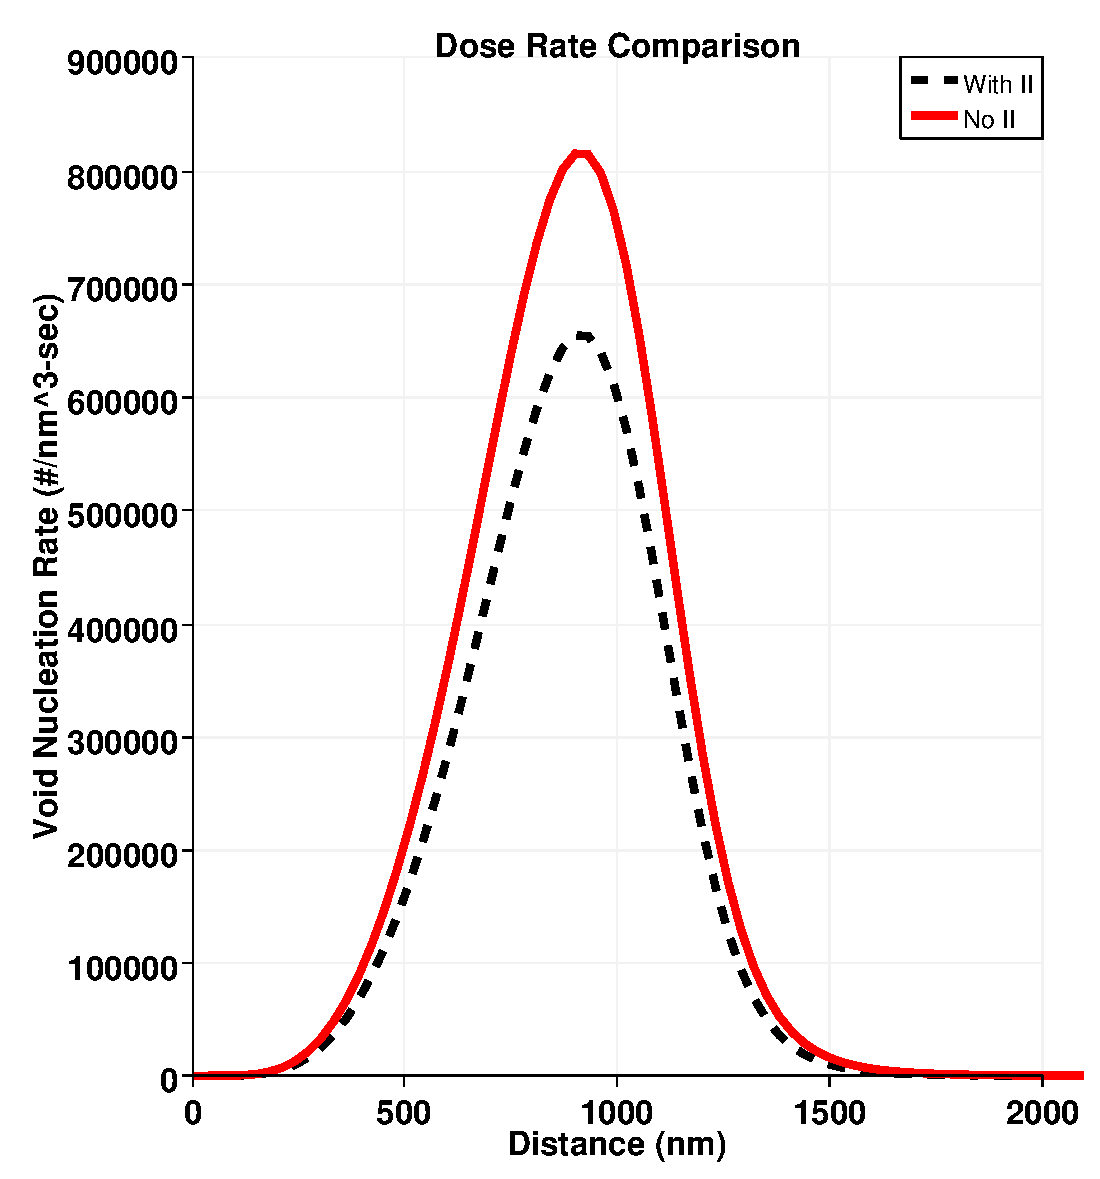
\includegraphics[width=0.9\columnwidth]{Figures/Dose-Rate-Comparison}
\par\end{centering}

\noindent \centering{}\protect\caption{\label{fig:Low-Dose-Rate}Void nucleation rate curves at a lower,
LWR-typical peak DPA rate of $\mathrm{10^{-7}\thinspace\frac{DPA}{sec}}$
for 3.5\,MeV $\mathrm{Fe^{++}}$ ions at 723K, showing no second
void nucleation rate peak. Injected interstitials (dashed black line)
do somewhat suppress the void nucleation rate, however.}
\end{figure}
Figure \ref{fig:Low-Dose-Rate} shows plots of void nucleation rate
in a typical dose rate of $\mathrm{10^{-7}\thinspace\frac{DPA}{sec}}$
found in a reactor. At this lower dose rate, no shifting in the peak
nucleation rate position is observed. This is due to the far lower
defect creation driving force compared to fixed sink strengths and
densities.

\begin{figure}
\noindent \begin{centering}
\includegraphics[width=1\columnwidth]{Figures/Temperature-Shift}
\par\end{centering}

\noindent \centering{}\protect\caption{\label{fig:Temperature-Shift}Normalized void nucleation rates for
3.5\,MeV $\mathrm{Fe^{+2}}$ irradiation of pure iron with injected
interstitials, at temperatures ranging from 673K to 773K}
\end{figure}
Injected interstitial effect strength was also studied at different
system temperatures, as summarized by Figure \ref{fig:Temperature-Shift}.
Prevalence of the sub-surface peak becomes more apparent at lower
temperatures. This is due to injected interstitials, which peak just
past the location of highest damage, locally suppressing vacancy concentration
as temperature decreases, and therefore decreasing local vacancy supersaturation.
Locations of both sub-surface and near-peak-damage maxima shift away
from the free surface with increasing temperature. For other ion energies
and DPA rates, the nucleation rate profiles will be different but
will preserve the features shown for 3.5\,MeV.

\begin{figure}
\noindent \begin{centering}
\includegraphics[width=1\columnwidth]{Figures/Ea-Comparison}
\par\end{centering}

\noindent \centering{}\protect\caption{\label{fig:Ea-Shift}Normalized void nucleation rates for 3.5\,MeV
$\mathrm{Fe^{+2}}$ irradiation of pure iron with injected interstitials,
at vacancy activation energies ranging fro 0.83-0.89\,eV}
\end{figure}
Finally, it was found that the behavior of the void nucleation rate
curve was extremely sensitive to changes in the vacancy migration
energy, the only tuning variable used in this study. Figure \ref{fig:Ea-Shift}
shows this dependence, in a narrow range from 0.83-0.89\,eV. The
fact that the results are so sensitive to this parameter implies that
precise knowledge of the vacancy migration energy, which is strongly
tied to ppm-level carbon impurities in iron \citep{Takaki1983}, may
determine whether the double-peak phenomenon is observed in a given
set of experimental or simulated conditions of dose rate, temperature,
and defect mobilities.


\section{Discussion}


\subsection{Importance of the Injected Interstitial Effect}

The results show qualitatively that the introduction of a subtle,
spatially-dependent defect imbalance may be responsible for significant
changes in both magnitude and shape of spatially dependent void distributions
evolving during ion irradiation. Injection of a very small fraction
of injected interstitials, never more than tenths of a percent, has
wide-reaching consequences. Interstitials are much more mobile, causing
increased recombination at the location of peak ballistic damage,
shifting the main damage peak towards the free surface by 100-200nm.
In addition, suppression of vacancy concentration by increased recombination
\textquotedblleft exposes\textquotedblright{} the second peak near
the free surface. This effect would not be seen without taking injected
interstitials into account.

This indicates that the injected interstitial effect, which has been
known for quite some time, must be accounted for when analyzing spatially
dependent void swelling experiments employing ion beam irradiation.
For example, \citep{Allen2005} and \citep{Cookson1993} mention irradiation
inducing ``nearly uniform damage,'' in this case referring to ballistic
radiation damage. A region of uniform resultant microstructural change
is unlikely to form, though the higher the energy of the bombarding
ion, the more uniform it may become in front of the ion stopping region.
More recent studies mention taking data from a region underneath the
surface, to avoid both the sub-surface and injected interstitial regions
\citep{Wang2015}. Small changes in parameters, such as temperature,
dose rate, and material purity (and therefore vacancy mobility) can
reveal or obscure the double peak, changing the relative magnitudes
of the injected interstitial and free surface effects. Care should
therefore be taken when interpreting such data from experiments. It
is therefore recommended to perform a spatially-dependent simulation
of defect concentrations during the irradiation experiment, to avoid
misinterpretation of data from a ``uniform region'' which may or
may not exist.

Modeling ion irradiation with and without injected interstitials at
varying temperatures shows the increasing importance of the injected
interstitials with decreasing vacancy mobility, as should be expected.
With increasing temperature, localization of injected interstitial
recombination decreases as both vacancies and interstitials become
more mobile. As vacancies increase in mobility, their ability to reach
the free surface from greater distances increases, shifting the sub-surface
peak away from the surface. In addition, as interstitials become more
mobile, they move farther on average before recombining or sinking,
spreading out their localized excess recombination effect.

These studies show that injected interstitial effects cannot be ignored
in simulations and experiments involving ion irradiation. Depending
on the temperature and the dose rate of irradiation, the resulting
vacancy supersaturation, and therefore the eventual void swelling
profile, can take on very different shapes. Over-generalization of
ion irradiation experiment behavior should therefore be remedied,
partially by taking this strong injected interstitial effect into
account.


\subsection{Shortcomings of the Model}

This model is deliberately simple, neglecting the formation of defect
clusters, dislocation forests, and other radiation defects which would
serve as additional point defect sinks. Initial simulations using
the model in this study clearly show, however, the injected interstitial
effect to weaken somewhat with increased sink density, which would
be expected to evolve as the material is irradiated. Therefore, a
quantitative measure of the injected interstitial effect will only
be possible by completely accounting for radiation-induced microstructural
changes, as proposed by Golubov et al. \citep{Golubov2012}. In addition,
the injected interstitial effect has been observed in far more complex
materials, even though the grain boundary and incoherent precipitate
sink terms are much stronger. In these alloys the observed swelling
vs, depth profiles show only the near-surface peak with total suppression
in the injected interstitial zone, most likely as a consequence of
their very high sink density. In simple materials such as iron (this
study), nickel, and even 316 stainless steel where the sink density
is much lower, ion irradiation usually, but not always, leads to a
double peak distribution \citep{Badger1985,Aruga1984,Bhattachary2014}
depending on the ion energy, DPA rate, and irradiation temperature.
In Badger's work \citep{Badger1985} the double peak in a very pure
316 model alloy moves from a double peak to a single peak as the temperature
is increased, as was observed in this study.

A full treatment of the injected interstitial effect in complex materials
may be possible by implementing extra, spatially-dependent interstitial
source terms found in recently developed models \citep{Barashev2014}.


\section{Conclusions}

A spatially varying rate theory model for radiation defect production
in ion-irradiated metals was modified to account for injected interstitials,
and augmented with some elements of the production bias model (PBM).
The presence of injected interstitials both suppresses and shifts
the main damage peak towards the free surface, while also reducing
the total vacancy supersaturation via increased recombination. This
\textquotedblleft exposes\textquotedblright{} a second peak, {\raise.17ex\hbox{$\scriptstyle\sim$}}200\,nm
from the free surface, which has been observed in recent experiments.
Predictions were made showing differences in the strength of this
effect at different temperatures and dose rates. The most important
observation is that the double peak behavior shifts with increasing
temperature to a single near-surface peak, in agreement with experimental
observations. The double peak is predicted only to be evident within
a narrow ({\raise.17ex\hbox{$\scriptstyle\sim$}}30C) temperature
window for self-ion irradiation of pure iron. Caution should be taken
when interpreting ion irradiation data, as the ballistic damage profile
may not match the resultant void swelling profile.

\bibliographystyle{unsrtnat}
\bibliography{InjectedInterstitials-NoTitles}

\end{document}
